\documentclass[12pt,a4paper,openright,twoside]{report}

\usepackage[italian]{babel}
\usepackage[utf8]{inputenc}
\usepackage{fancyhdr}
\usepackage{float}

% libreria per avere l'indentazione all'inizio dei capitoli
\usepackage{indentfirst}

% libreria per mostrare le etichette
%\usepackage{showkeys}

% libreria per inserire grafici
\usepackage{graphicx}

% libreria per utilizzare font particolari, ad esempio \textsc{}
\usepackage{newlfont}

% librerie matematiche
\usepackage{amssymb} \usepackage{amsmath}
\usepackage{latexsym}
\usepackage{amsthm}
\usepackage{cite}
\usepackage{listings}
\usepackage{hyperref}
\usepackage[square,numbers,sort]{natbib}
\usepackage{xcolor}

% \bibliographystyle{unsrt}
\bibliographystyle{unsrtnat}

\lstset{
    frame=single,
    breaklines=true
}

\oddsidemargin=30pt
\evensidemargin=20pt

% serve per la sillabazione: tra parentesi vanno inserite come nell'esempio le
% parole che latex non riesce a tagliare nel modo giusto andando a capo.
\hyphenation{sil-la-ba-zio-ne pa-ren-te-si}

% comandi per l'impostazione della pagina
\pagestyle{fancy}
\addtolength{\headwidth}{20pt}
\renewcommand{\chaptermark}[1]{\markboth{\thechapter.\ #1}{}}
\renewcommand{\sectionmark}[1]{\markright{\thesection \ #1}{}}
\rhead[\fancyplain{}{\bfseries\leftmark}]{\fancyplain{}{\bfseries\thepage}}
\cfoot{}

% comando per impostare l'interlinea
\linespread{1.3}

\newcommand{\xstudent}{CHRISTIAN RICCI}
\newcommand{\xsupervisor}{MORENO MARZOLLA}




\begin{document}

% scelta delle dimensioni della pagina
%\setlength{\textwidth}{13.5cm}
%\setlength{\textheight}{19cm}
%\setlength{\footskip}{3cm}

% %%% inizio prefazione %%%

%\textwidth=450pt
\oddsidemargin=25pt

\begin{titlepage}
\begin{center}
    {\Large{\textsc{Alma Mater Studiorum}}}\\
    {\Large{\textsc{Universit\`a di Bologna}}} \\
    {\textsc{Campus di Cesena}}
    % thin and big line
    \rule[0.1cm]{14cm}{0.1mm}
    \rule[0.5cm]{14cm}{0.6mm}
    DIPARTIMENTO DI INFORMATICA – SCIENZA E INGEGNERIA
    Corso di Laurea in Ingegneria e Scienze Informatiche
\end{center}

\vspace{15mm}

\begin{center}
    {\LARGE{\bf STEREOMATCHING SU GPU}} \\
\end{center}

\vspace{15mm}

\begin{center}
     \large{ Elaborato in:\\ High Performance Computing\\}
\end{center}

\vspace{20mm}
\par
\noindent

\begin{minipage}[t]{0.47\textwidth}
    {\large{\bf Relatore:\\ Prof.\\ \xsupervisor}}
\end{minipage}
\hfill
\begin{minipage}[t]{0.47\textwidth}\raggedleft
    {\large{\bf Presentata da:\\ \xstudent}} \end{minipage}
\vspace{20mm}
% TODO anno e sessione
\begin{center}
    \large{\bf Sessione I\\ Anno Accademico 2022-2023}
\end{center}
\end{titlepage}

\clearpage{\pagestyle{empty}\cleardoublepage}

\newpage

% %%% pagina della dedica %%%
\begin{titlepage}
\thispagestyle{empty}
\topmargin=6.5cm
\raggedleft
\large
\em
(Dedica)
\clearpage{\pagestyle{empty}\cleardoublepage}
\end{titlepage}

% %%% indice %%%

\pagenumbering{roman}

\tableofcontents
\rhead[\fancyplain{}{\bfseries\leftmark}]{\fancyplain{}{\bfseries\thepage}}
\lhead[\fancyplain{}{\bfseries\thepage}]{\fancyplain{}{\bfseries INDICE}}
\clearpage{\pagestyle{empty}\cleardoublepage}

\listoffigures
\clearpage{\pagestyle{empty}\cleardoublepage}

%\listoftables
%\clearpage{\pagestyle{empty}\cleardoublepage}

\pagenumbering{arabic}



\chapter*{Introduzione}

% imposta l'intestazione di pagina
\rhead[\fancyplain{}{\bfseries INTRODUZIONE}]{\fancyplain{}{\bfseries\thepage}}
\lhead[\fancyplain{}{\bfseries\thepage}]{\fancyplain{}{\bfseries INTRODUZIONE}}

% aggiunge la voce Introduzione nell'indice
\addcontentsline{toc}{chapter}{Introduzione}

La \textit{Stereo Vision} è un popolare argomento di ricerca nel campo della Visione Artificiale; esso consiste nell\'usare due immagini di una stessa scena, prodotte da due fotocamere diverse, per estrarre informazioni in 3D. L\'idea di base della \textit{Stereo Vision} è la simulazione della visione binoculare umana: le due fotocamere sono disposte in orizzontale per fungere da ``occhi'' che guardano la scena in 3D. Confrontando le due immagini ottenute, si possono ottenere informazioni riguardo alle posizioni degli oggetti della scena.

In questa relazione presenteremo un algoritmo di Stereo Vision: si tratta di un algoritmo parallelo che ha come obiettivo di tracciare le linee di livello di un area geografica. L\'algoritmo in genesi era stato implementato per la \textit{Connection Machine CM-2}, un supercomputer sviluppato negli anni 80, ed era espresso in \textbf{*Lisp}, un linguaggio derivato dal Lisp e ideato per la macchina stessa.

Questa relazione tratta anche la traduzione e l\'implementazione dell\'algoritmo in \textbf{CUDA}, ovvero un\'architettura hardware per l\'elaborazione parallela sviluppata da NVIDIA, che consente di eseguire codice parallelo su GPU. Si darà inoltre uno sguardo alle difficoltà che sono state riscontrate nella traduzione da *Lisp a CUDA.



\rhead[\fancyplain{}{\bfseries\leftmark}]{\fancyplain{}{\bfseries\thepage}}
\lhead[\fancyplain{}{\bfseries\thepage}]{\fancyplain{}{\bfseries INDICE}}
\clearpage{\pagestyle{empty}\cleardoublepage}
\clearpage{\pagestyle{empty}\cleardoublepage}
\chapter{Programmazione Parallela}

\lhead[\fancyplain{}{\bfseries\thepage}]{\fancyplain{}{\bfseries\rightmark}}

La programmazione parallela è un paradigma di programmazione che sfrutta l\'esecuzione parallela di processori per ottenere prestazioni migliori e risultati nel minor tempo possibile. I calcoli vengono eseguiti in parallelo, ovvero vengono eseguiti simultaneamente su più processi. Questo paradigma si colloca all\'interno dell\'High Performance Computing (HPC), una materia che studia le tecniche e soluzioni hardware che facilitano l\'esecuzione parallela dei calcoli.



\section{Evoluzione dei Processi}

Perchè mai si dovrebbe ricorrere all\'esecuzione parallela per ottenere prestazioni migliori? Questa domanda trova risposta nello studio dell'evoluzione dei processori: per anni si è tenuto conto della cosiddetta ``Legge di Moore'', che ipotizza che ``il numero di transistor contenuti all'interno di un chip raddoppia ogni due anni''. Questa legge fu enunciata da Gordon E. Moore nel 1965 e spiega che effettivamente le prestazioni di un chip si duplicavano ogni due anni. La sua osservazione si rivelò corretta per due decenni, ma intorno agli anni 2000 questo andamento iniziò a calare. I motivi principali di questo calo sono:

\begin{itemize}
    \item La dimensione dei transistor. Il miglior modo per aumentare il numero di transistor è di renderli sempre più piccoli, ma esiste un limite fisico della grandezza minima. I transistor di oggi vanno dai 20 nm all'1 nm;
    \item Il calore dissipato dal processore. Un processore più veloce corrisponde ad una più grande quantità di calore dissipato, che porta a problemi di instabilità nel processore.
\end{itemize}

Al posto di aumentare il numero di transistor, negli ultimi due decenni sono state ideate nuove architetture che sfruttano il parallelismo: queste sono le architetture parallele, anche chiamate multicore o multiprocessore. Queste architetture sono sviluppate aggiungendo più processori logici dentro ad un chip. Le prestazioni che si possono ottenere con le architetture parallele derivano quindi dalla suddivisione del lavoro che è distribuito in più unità operazionali.

\begin{figure}[h]
\centering{}
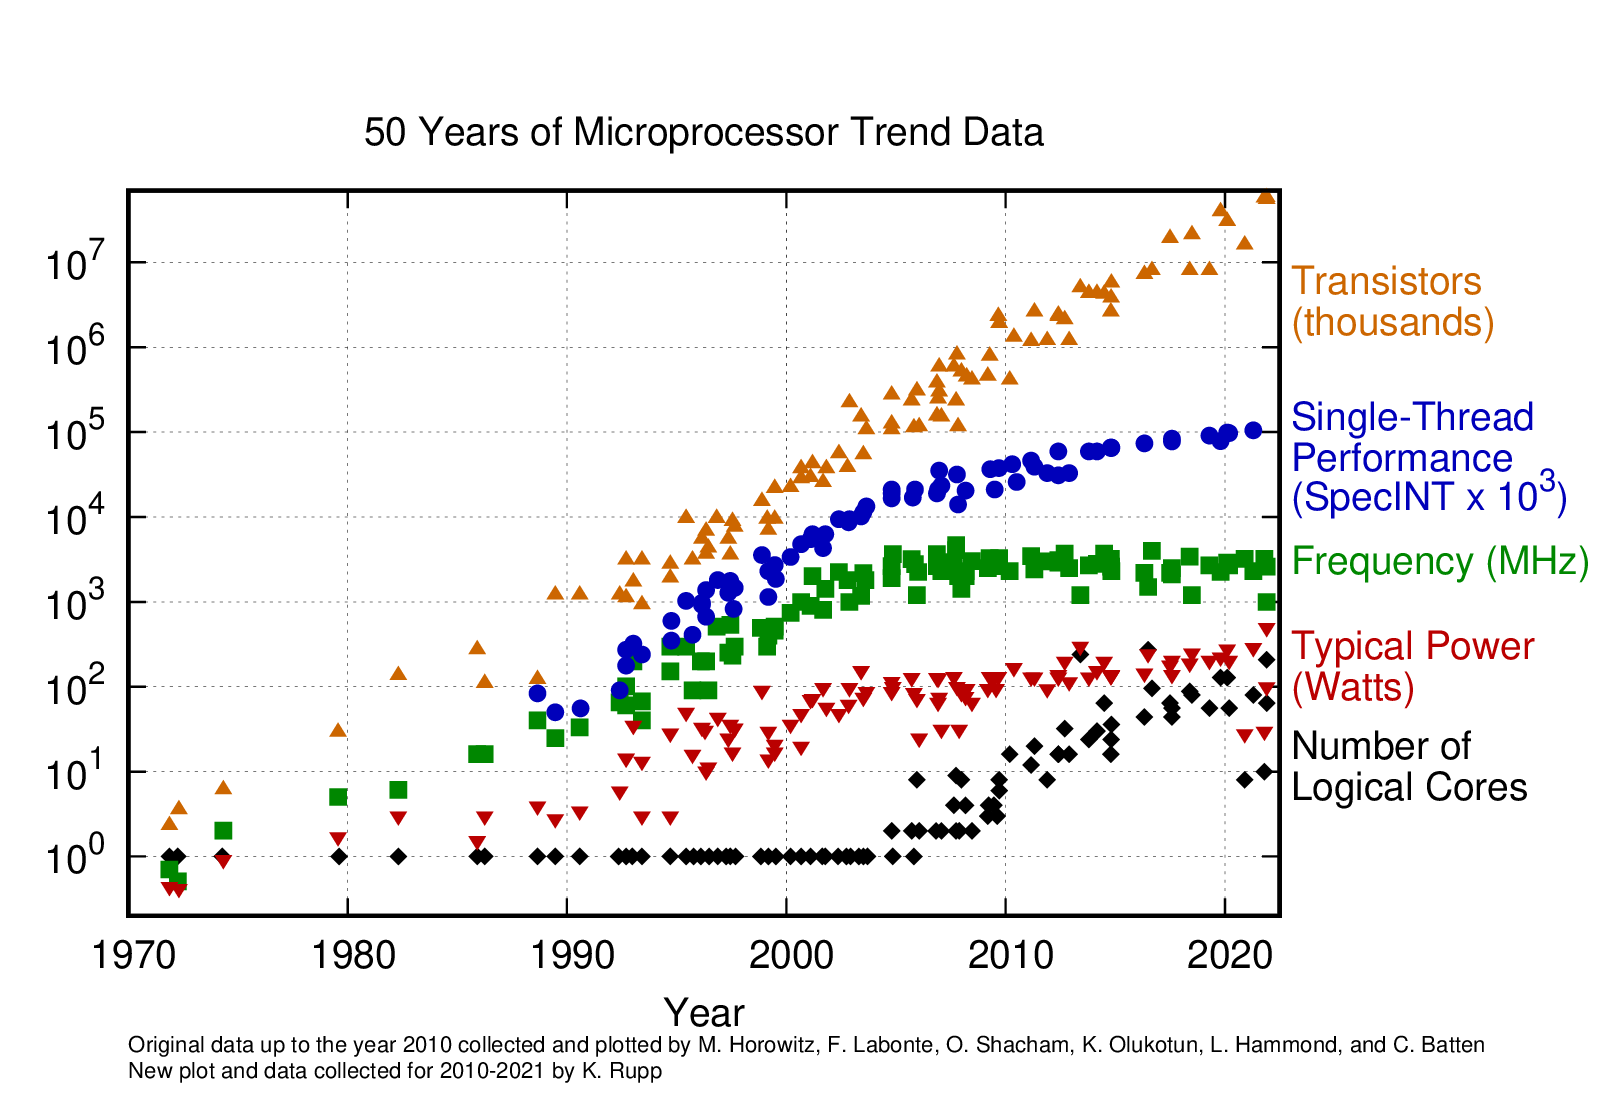
\includegraphics[width=\textwidth]{50-years-processor-trend.png}
\caption{Evoluzione delle caratteristiche dei processori}
\label{img:trend_proc}
\end{figure}

Nella figura \ref{img:trend_proc} viene mostrata l'evoluzione dei processori nel corso degli ultimi decenni. In particolare, si può notare come la frequenza media dei processori si sia stabilizzata, mentre più o meno dalla metà degli anni 2000 sia cresciuto il numero di core logici, a seguito di ricerche sullo sviluppo delle architetture parallele.

\section{GPU e CUDA}

Esistono diverse tipologie di architetture parallele; in questa relazione ci interesseremo delle architetture basate su GPU. Queste architetture vengono chiamate GPGPU (General Purpose Graphics Processing Units), ovvero schede grafiche programmabili in maniera generica.

\begin{figure}[h]
\centering{}
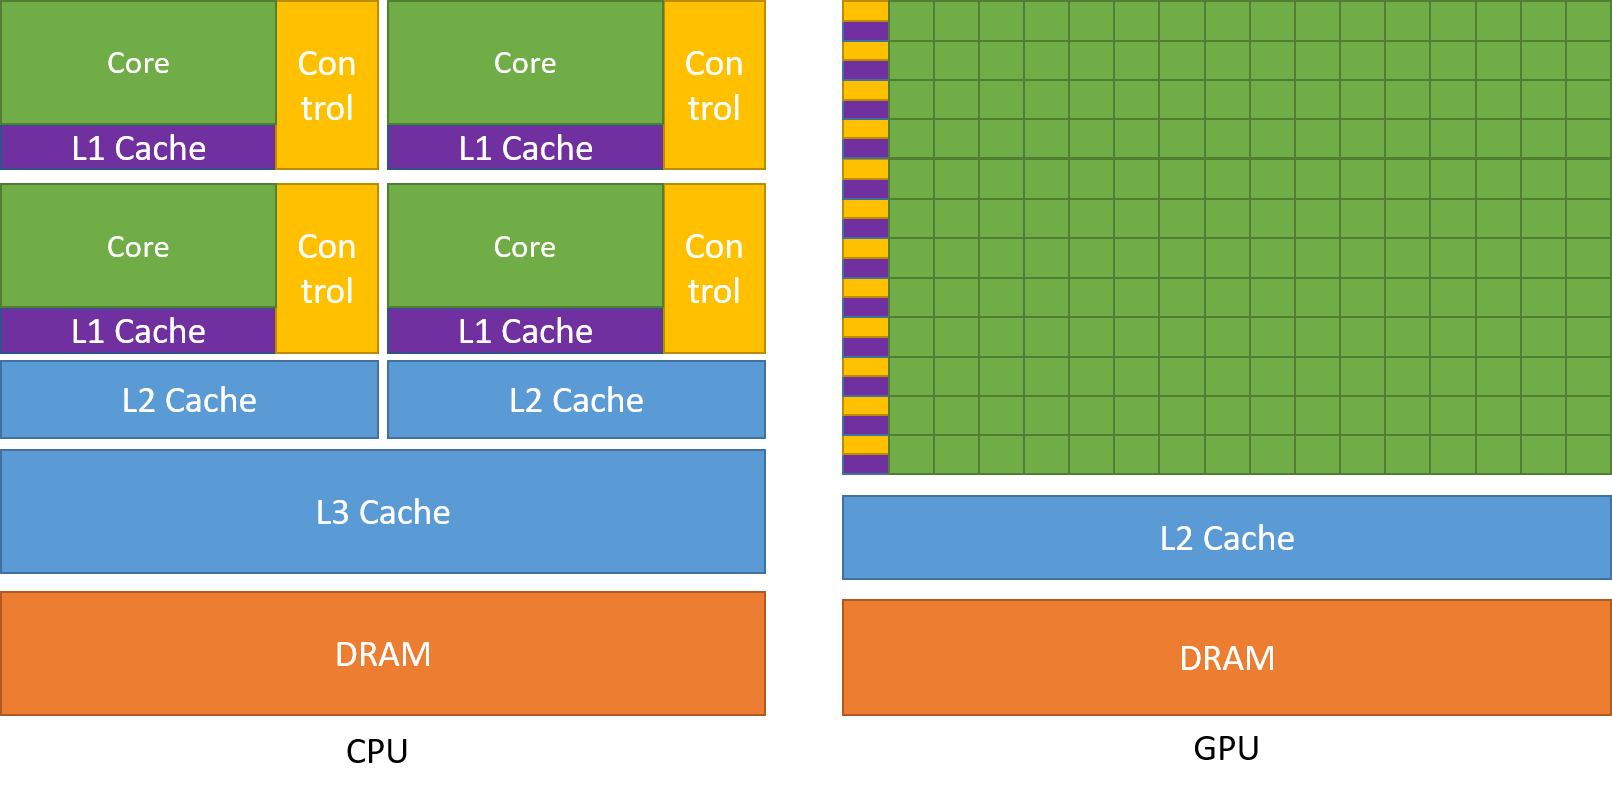
\includegraphics[width=\textwidth]{cpu-gpu-comparison.png}
\caption[Confronto tra CPU e GPU]{Confronto tra l'architettura di una CPU e quella di una GPU. Da notare l'elevato numero di core della GPU.}
\label{img:cpu-gpu-comparison}
\end{figure}

Il nome di queste architetture potrebbe dare confusione dato che, in generale, la funzione di una scheda video è strettamente legata alla grafica. Il motivo per cui sono interessanti è per la presenza di un grande numero di core all'interno della scheda, molto più grande del numero di core presenti in una normale CPU (si tratta di due ordini di grandezza di differenza); questo implica che possono essere molto utili per programmi paralleli con dati di grandi dimensioni. Le prime ricerche a riguardo furono svolte nel 2001 e nel 2003; diventarono più popolari nel 2007 con l'avvento di CUDA.

CUDA (Compute Unified Device Architecture) è una piattaforma per il calcolo parallelo sviluppata da NVIDIA. Si tratta di una piattaforma che consente l'utilizzo delle schede grafiche NVIDIA per eseguire programmi paralleli, sfruttando appieno le loro potenzialità. La prima versione di CUDA è stata pubblicata nel 2007.

I concetti di base di CUDA sono molto semplici: CUDA prevede una separazione tra l'\textit{host}, che corrisponde la CPU, e il \textit{device}, che corrisponde ad una o più schede grafiche. Queste sono considerate unità indipendenti, che cooperano in modo asincrono: in particolare, l'\textit{host} ha la possibilità di invocare funzioni specifiche che vengono eseguite sul \textit{device}. Queste funzioni vengono dette \textit{kernel}; appena vengono chiamate, queste vengono eseguite asincronicamente e restituiscono subito il controllo all'\textit{host}.

\subsection{Architettura di CUDA}

\begin{figure}[h]
\centering{}
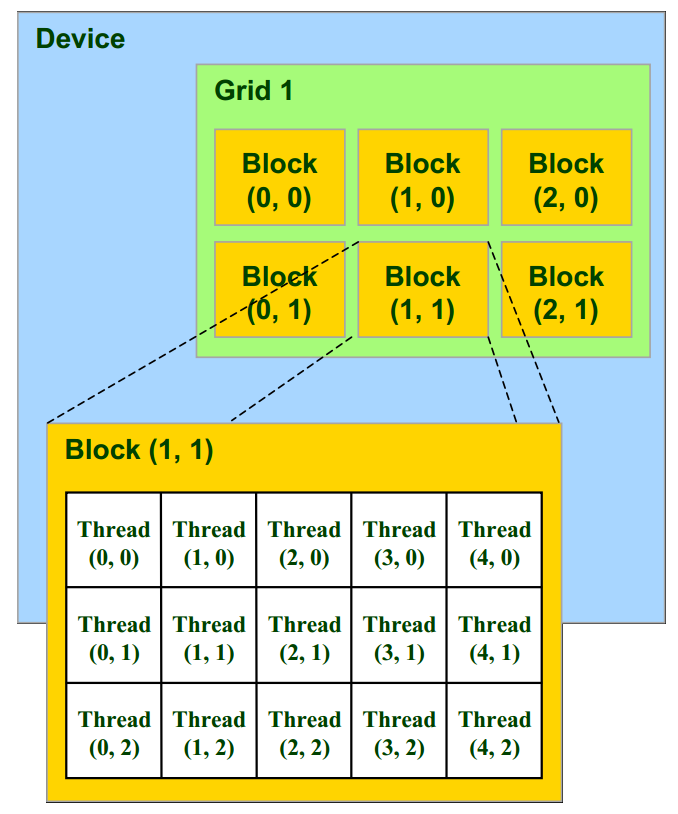
\includegraphics[width=6.5cm]{grids-and-blocks.png}
\caption{Gerarchia dei thread in CUDA}
\label{img:grids-and-blocks}
\end{figure}

In CUDA, l'unità minima di elaborazione è il \textbf{thread}. CUDA raggruppa logicamente i thread in più \textbf{blocchi}, e a loro volta i blocchi sono raggruppati in \textbf{griglie}.

Un blocco è considerato un unità indipendente di lavoro: esso può avere una, due o tre dimensioni, il che significa che può essere indicizzato in più dimensioni in base all'occorrenza; ogni blocco può essere eseguito in qualunque ordine all'interno di una griglia. Il numero di thread in un blocco è limitato a va fino a 1024 thread per blocco.

Una griglia rappresenta un lavoro affidato alla GPU: anch'esso può essere tridimensionale e non ha limiti sul numero di blocchi.

Lo \textbf{scheduling dei thread} in CUDA è completamente automatico: non è possibile scegliere quali e quanti core (che in CUDA vengono chiamati \textit{Streaming Multiprocessor} debbano venire utilizzati.

\subsection{Struttura e gestione della memoria}

Quando si scrive un \textit{kernel}, non ci si deve mai preoccupare di come vengono gestiti i thread. Sarà l\'hardware stesso a preoccuparsi, durante l\'esecuzione, di effettuare lo scheduling migliore sfruttando al massimo l\'hardware: in particolare, in CUDA esiste il concetto di \textit{warp}, che rappresenta l\'unità minima di schedulazione e contiene un certo numero di thread (massimo 32). L\'hardware raggruppa assieme in un \textit{warp} i thread che devono eseguire la stessa porzione di codice; i thread eseguono le istruzioni seguendo il paradigma SIMD.

\begin{figure}[h]
\centering{}
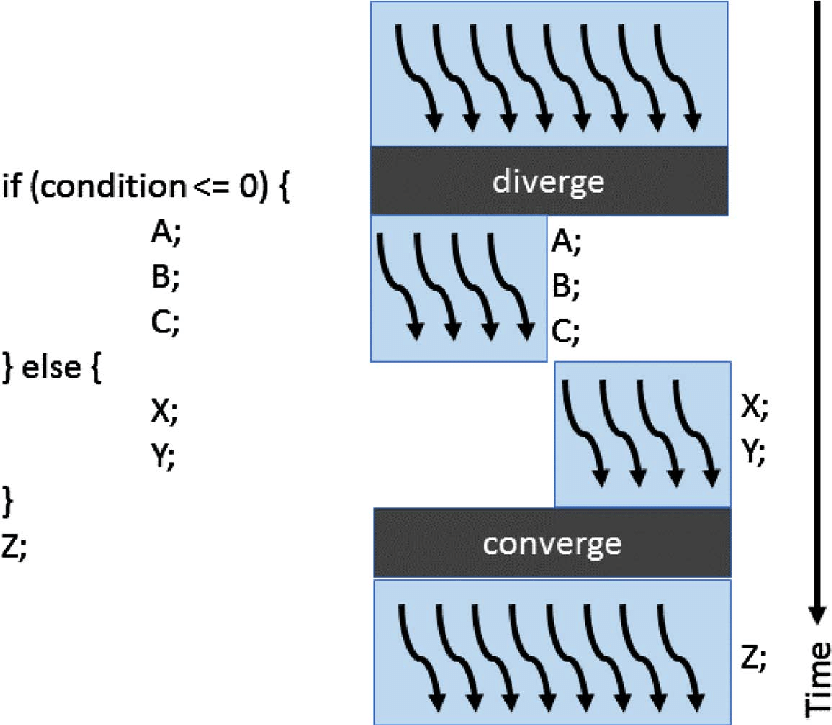
\includegraphics[width=6.5cm]{warp-branch.png}
\caption{Esecuzione di un thread in caso di biforcazione}
\label{img:warp-branch}
\end{figure}

Nel caso ci sia una biforcazione nel flusso di controllo (causato, ad esempio, da costrutti if-else), la condizione viene calcolata per ogni thread, dopodichè vengono eseguiti i thread per cui è stata verificata, mentre gli altri rimangono fermi. L'hardware comunque può trasferire i thread che sono rimasti fermi in altri warp.

\newpage

La memoria in CUDA, riassunta nella figura \ref{img:memory-hierarchy}, è suddivisa in più tipi:

\begin{itemize}
    \item \textbf{Memoria globale}: è la memoria più grande (alcuni GB). A questa memoria possono accedervi ogni thread di ogni blocco, ma presenta una latenza di accesso più alta;
    \item \textbf{Memoria delle constanti}: una memoria persistente anch\'essa accessibili da ogni thread, ma ci si può accedere in sola lettura. È più piccola, di soli 64 KB;
    \item \textbf{Memoria texture}: un'altra memoria di sola lettura e accessibile da tutti, ma è ottimizzata per le texture;
    \item \textbf{Memoria condivisa}: è una memoria molto veloce che viene condivisa tra tutti i thread di un solo blocco. Per blocco ci sono 48 KB di memoria condivisa;
    \item \textbf{Memoria locale}: una memoria dedicata per ogni thread, accessibile solo da esso. Non persiste tra l'esecuzione di due kernel;
\end{itemize}

\begin{figure}[h]
    \centering
    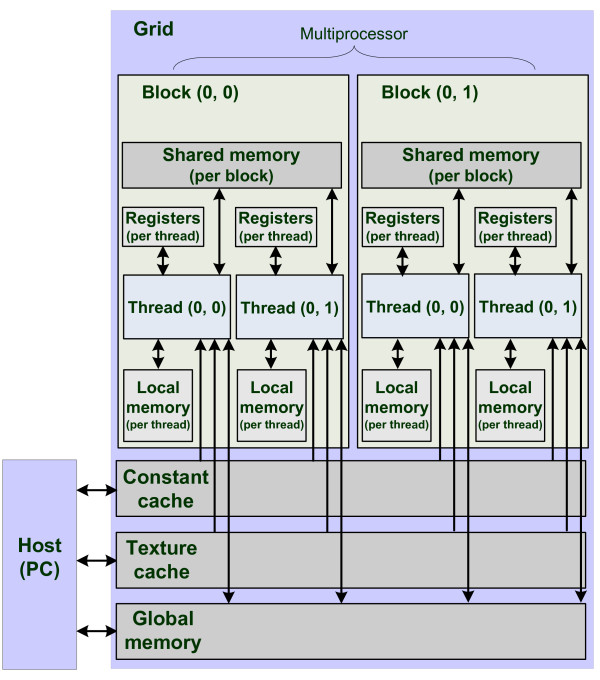
\includegraphics[width=8cm]{cuda-memory-hierarchy.jpg}
    \caption{La struttura della memoria in CUDA.}
    \label{img:memory-hierarchy}
\end{figure}

In CUDA va prestata particolare attenzione all'accesso della memoria. Infatti, quando un thread esegue un accesso alla memoria anche molto piccolo (4 byte), la GPU legge almeno 32 byte consecutivi. Una caratteristica molto importante è il \textbf{raggruppamento degli accessi}: se più thread accedono a posizioni di memoria consecutive, la GPU raggruppa questi accessi in una sola lettura.

\begin{figure}
    \centering
    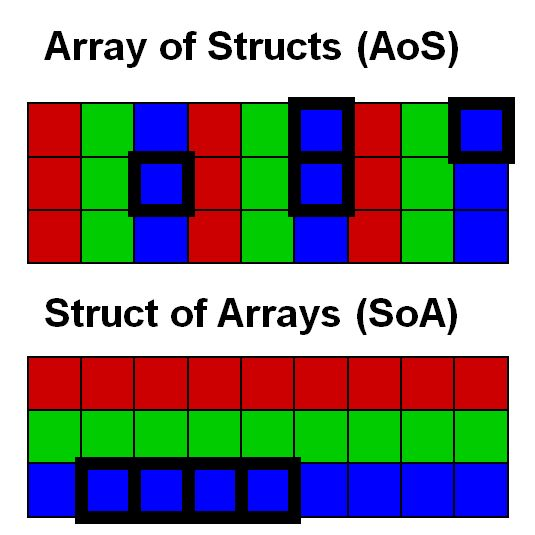
\includegraphics[width=5cm]{aos.jpg}
    \caption{AoS e SoA a confronto}
    \label{img:aos}
\end{figure}

Questo in pratica significa che in CUDA il pattern di memorizzazione classico, ovvero l'Array-of-Structures, non è adeguato e si dovrebbe preferire la Structure-of-Arrays. Il primo consiste nel conversare i dati di un elemento (ad esempio un punto con coordinate x, y e z) in posizioni adiacenti di memoria: di conseguenza, un array di punti consisterà in un array di coordinate (x, y, z) che si ripete per ogni punto. Il secondo consiste nell'avere un array per ogni dato dell'elemento: si avrà un array per ogni coordinata X, coordinata Y e coordinata Z. La figura \ref{img:aos} mostra un confronto visuale dei due pattern.

Immaginiamo di avere più thread che devono leggere ognuno le coordinate X di ogni punto. Se i dati sono memorizzati mediante AoS, i valori in sè sarebbero più lontani tra loro, con conseguenza maggiori letture e maggior utilizzo del bus. Al contrario, con SoA si avrebbe tutti elementi adiacenti e si avrebbe bisogno di meno letture.

\subsection{Il linguaggio CUDA}

Per scrivere un kernel, CUDA prevede un apposito linguaggio: il linguaggio che si usa è un estensione del C e del C++ con l'aggiunta di parole chiave ed altre caratteristiche per facilitare la scrittura del codice per GPU.

In particolare, CUDA aggiunge le seguenti parole chiave per le funzioni:

\begin{itemize}
    \item \verb|__host__|: usata per funzioni scritte per la CPU (presente di default se non ci sono altre parole chiave di CUDA);
    \item \verb|__device__|: usata per le funzioni scritte per la GPU e chiamate dalla GPU;
    \item \verb|__global__|: usata per le funzioni scritte per la GPU, ma chiamate dalla CPU. In essenza sono il punto d'entrata tra codice dell'\textit{host} e codice del \textit{device};
\end{itemize}

\verb|__host__| e \verb|__device__| possono essere combinati assieme. CUDA aggiunge anche le seguenti parole chiave per le variabili:

\begin{itemize}
    \item \verb|__constant__|: piazza la variabile in memoria costante;
    \item \verb|__device__|: piazza la variabile nella memoria globable della GPU. Essa è comunque accessibile dall\'host tramite opportune funzioni;
    \item \verb|__shared__|: piazza la variabile nella memoria shared. In questo caso, il suo accesso è limitato al singolo blocco;
\end{itemize}

L\'estensione più importante in CUDA riguarda il modo in cui si chiamano le funzioni dichiarate \verb|__global__|:

\chapter{Stereo Vision}

secondo capitolo.



\chapter{Connection Machine e *Lisp}

il terzo capitolo.



\chapter{Descrizione dell'algoritmo}



\chapter{Progettazione}

capitolo 4



\chapter{Metriche di valutazione}

\chapter{Valutazione delle prestazioni}

\chapter*{Conclusioni}

\rhead[\fancyplain{}{\bfseries CONCLUSIONI}]{\fancyplain{}{\bfseries\thepage}}
\lhead[\fancyplain{}{\bfseries\thepage}]{\fancyplain{}{\bfseries CONCLUSIONI}}

\addcontentsline{toc}{chapter}{Conclusioni}
Queste sono le conclusioni.\\



% %%% bibliografia %%%

\clearpage{\pagestyle{empty}\cleardoublepage}

\rhead[\fancyplain{}{\bfseries BIBLIOGRAFIA}]{\fancyplain{}{\bfseries\thepage}}
\lhead[\fancyplain{}{\bfseries\thepage}]{\fancyplain{}{\bfseries BIBLIOGRAFIA}}

\bibliography{biblio}{}
\bibliographystyle{plain}

\addcontentsline{toc}{chapter}{Bibliografia}

\rhead[\fancyplain{}{\bfseries \leftmark}]{\fancyplain{}{\bfseries\thepage}}
\clearpage{\pagestyle{empty}\cleardoublepage}



\chapter*{Ringraziamenti}
\addcontentsline{toc}{chapter}{Ringraziamenti}
\thispagestyle{empty}
Ringraziamenti.

\nocite{*}

\end{document}
